\documentclass[12pt]{article}
\input{/Users/circle/Documents/博一下/homework/setting.tex}
\setcounter{secnumdepth}{2}
\usepackage{bm}
\usepackage{autobreak}
\usepackage{amsmath}
\setlength{\parindent}{2em}
\graphicspath{{../}}

%pdf文件设置
\hypersetup{
	pdfauthor={袁磊祺},
	pdftitle={统计力学及应用作业4}
}

\title{
		\vspace{-1in} 	
		\usefont{OT1}{bch}{b}{n}
		\normalfont \normalsize \textsc{\LARGE Peking University}\\[1cm] % Name of your university/college \\ [25pt]
		\horrule{0.5pt} \\[0.5cm]
		\huge \bfseries{统计力学及应用作业4} \\
		\horrule{2pt} \\[0.5cm]
}
\author{
		\normalfont 								\normalsize
		College of Engineering \quad 2001111690  \quad 袁磊祺\\	\normalsize
        \today
}
\date{}

\begin{document}

\input{setc.tex}

\maketitle

\section{1}

根据教材的(15.8)有
\begin{equation}
	S=-\left(\frac{\partial G}{\partial T}\right)_P,\quad V = \left(\frac{\partial G}{\partial P}\right)_T.
\end{equation}
又根据
\begin{gather}
	G = E-TS+PV,\\
	G=F+PV,\\
	G=H-TS.
\end{gather}
得
\begin{gather}
	E=G-T\left(\frac{\partial G}{\partial T}\right)_P+P\left(\frac{\partial G}{\partial P}\right)_T,\\
	F=G-P\left(\frac{\partial G}{\partial P}\right)_T,\\
	H=G-T\left(\frac{\partial G}{\partial T}\right)_P.
\end{gather}

又
\begin{equation}
	C_p = \left(\frac{\partial H}{\partial T}\right)_P = \left(\frac{\partial \left(G-T\left(\frac{\partial G}{\partial T}\right)_P\right)}{\partial T}\right)_P.
\end{equation}
\begin{equation}
	C_v=C_p+T\frac{\left(\frac{\partial V}{\partial T}\right)^2_P}{\left(\frac{\partial V}{\partial P}\right)_T}=\left(\frac{\partial \left(G-T\left(\frac{\partial G}{\partial T}\right)_P\right)}{\partial T}\right)_P+T\frac{\left(\frac{\partial \left(\frac{\partial G}{\partial P}\right)_T}{\partial T}\right)^2_P}{\left(\frac{\partial \left(\frac{\partial G}{\partial P}\right)_T}{\partial P}\right)_T}.
\end{equation}\qed


\section{2}


\begin{align}
	C_{p} & =T\left(\frac{\partial S}{\partial T}\right)_{P}=T \frac{\partial(S, P)}{\partial(T, P)}=T \frac{\partial(S, P) / \partial(T, V)}{\partial(T, P) / \partial(T, V)}                                                                                  \\
	      & =T \frac{\left(\frac{\partial S}{\partial T}\right)_{V}\left(\frac{\partial P}{\partial V}\right)_{T}-\left(\frac{\partial S}{\partial V}\right)_{T}\left(\frac{\partial P}{\partial T}\right)_{V}}{\left(\frac{\partial P}{\partial V}\right)_{T}} \\
	      & =C_{v}-T \frac{\left(\frac{\partial S}{\partial V}\right)_{T}\left(\frac{\partial P}{\partial T}\right)_{V}}{\left(\frac{\partial P}{\partial V}\right)_{T}}                                                                                        \\
	      & =C_v - T  \frac{\left(\frac{\partial P}{\partial T}\right)_{V}^2}{\left(\frac{\partial P}{\partial V}\right)_{T}},
\end{align}
即
\begin{equation}
	C_{p} - C_v = - T  \frac{\left(\frac{\partial P}{\partial T}\right)_{V}^2}{\left(\frac{\partial P}{\partial V}\right)_{T}}.\qed
\end{equation}

\section{3}

\subsection{1}

不能,只能通过状态方程求出$C_p,\ C_v$的差。

\subsection{2}

通过测量$C_p$或$C_v$,然后积分
\begin{equation}
	C_v = T \left(\frac{\partial S}{\partial T}\right)_V
\end{equation}
得$S$,然后通过积分
\begin{equation}
	\dif E = T \dif S - P \dif V,
\end{equation}
得$E$,然后可得
\begin{gather}
	G = E-TS+PV,\\
	F=E-TS,\\
	H=E+PV.
\end{gather}

\subsection{3}

在$V$不变的情况下
\begin{equation}
	E = \int_0^T C_v(\tau)\tau \dif \tau,
\end{equation}
\begin{equation}
	S = \int_0^T C_v(\tau)/\tau \dif \tau.
\end{equation}

\begin{gather}
	G = \int_0^T C_v(\tau)\tau \dif \tau-T\int_0^T C_v(\tau)/\tau \dif \tau+PV,\\
	F=\int_0^T C_v(\tau)\tau \dif \tau-T\int_0^T C_v(\tau)/\tau \dif \tau,\\
	H=\int_0^T C_v(\tau)\tau \dif \tau+PV.
\end{gather}


\section{4}

一个一维简谐振子与一个温度为$\tau$的热库相互作用,简谐振子$H=\frac{p^2}{2}+\frac{x^2}{2},\ \tau = 1.5$(无量纲单位)。用 Metropolis 方法求相空间分布$\rho(x,p)$.

\begin{enumerate}
	\item 相点初始位置为$(0,0)$.
	\item 若相点在某一点$x_1$,则在两个方向都产生一个位移,步长为$[0,6]$中的一个随机数,到达点$x_2$.
	\item 根据
	      \begin{equation}
		      E = \me^{-H/\tau}
	      \end{equation}
	      来计算其概率密度。
	      \begin{enumerate}
		      \item 若$E_2>E_1$,则相点移动到$x_2$。
		      \item 若$E_2<E_1$,则产生一个$[0,1]$中的随机数$\xi$,若$\xi<\me^{-(H_2-H_1)/\tau}$则相点移动到$x_2$。否则不移动。
	      \end{enumerate}
	\item 重复2,3,直到给定的停止条件。
\end{enumerate}

\cref{fig:1} 为散点分布图,可以发现粒子处于原点的概率最大.\cref{fig:2} 为二维概率密度分布图,即$\rho(x,p)$.







\begin{figure}[htp]
	\centering
	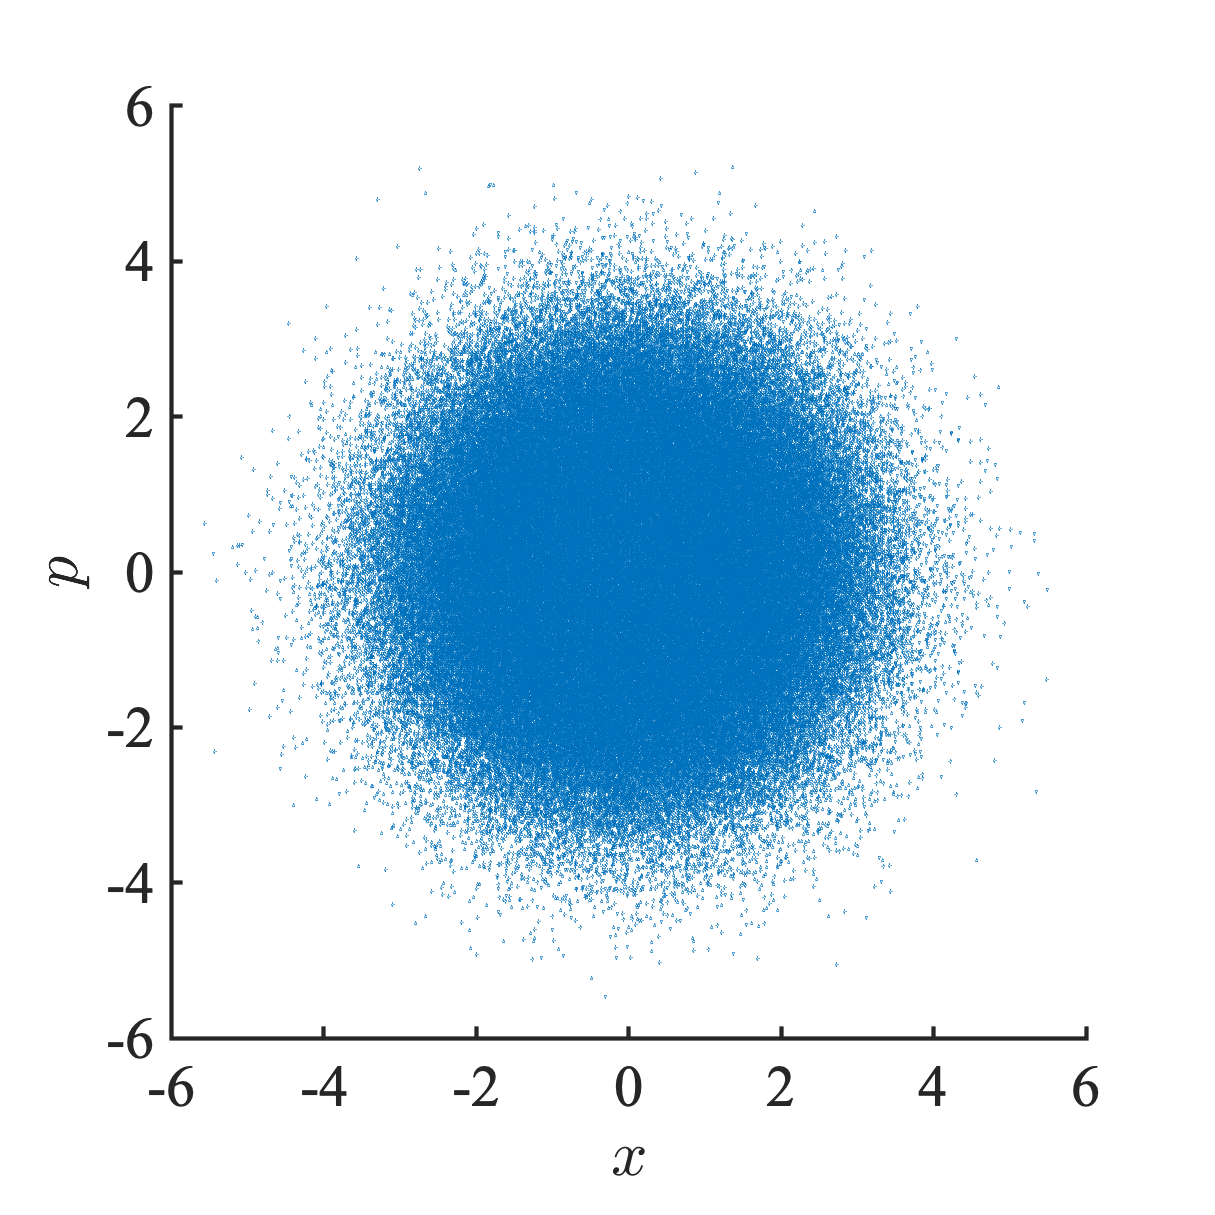
\includegraphics[width=9cm]{1.eps}
	\caption{散点图.}
	\label{fig:1}
\end{figure}


\begin{figure}[htp]
	\centering
	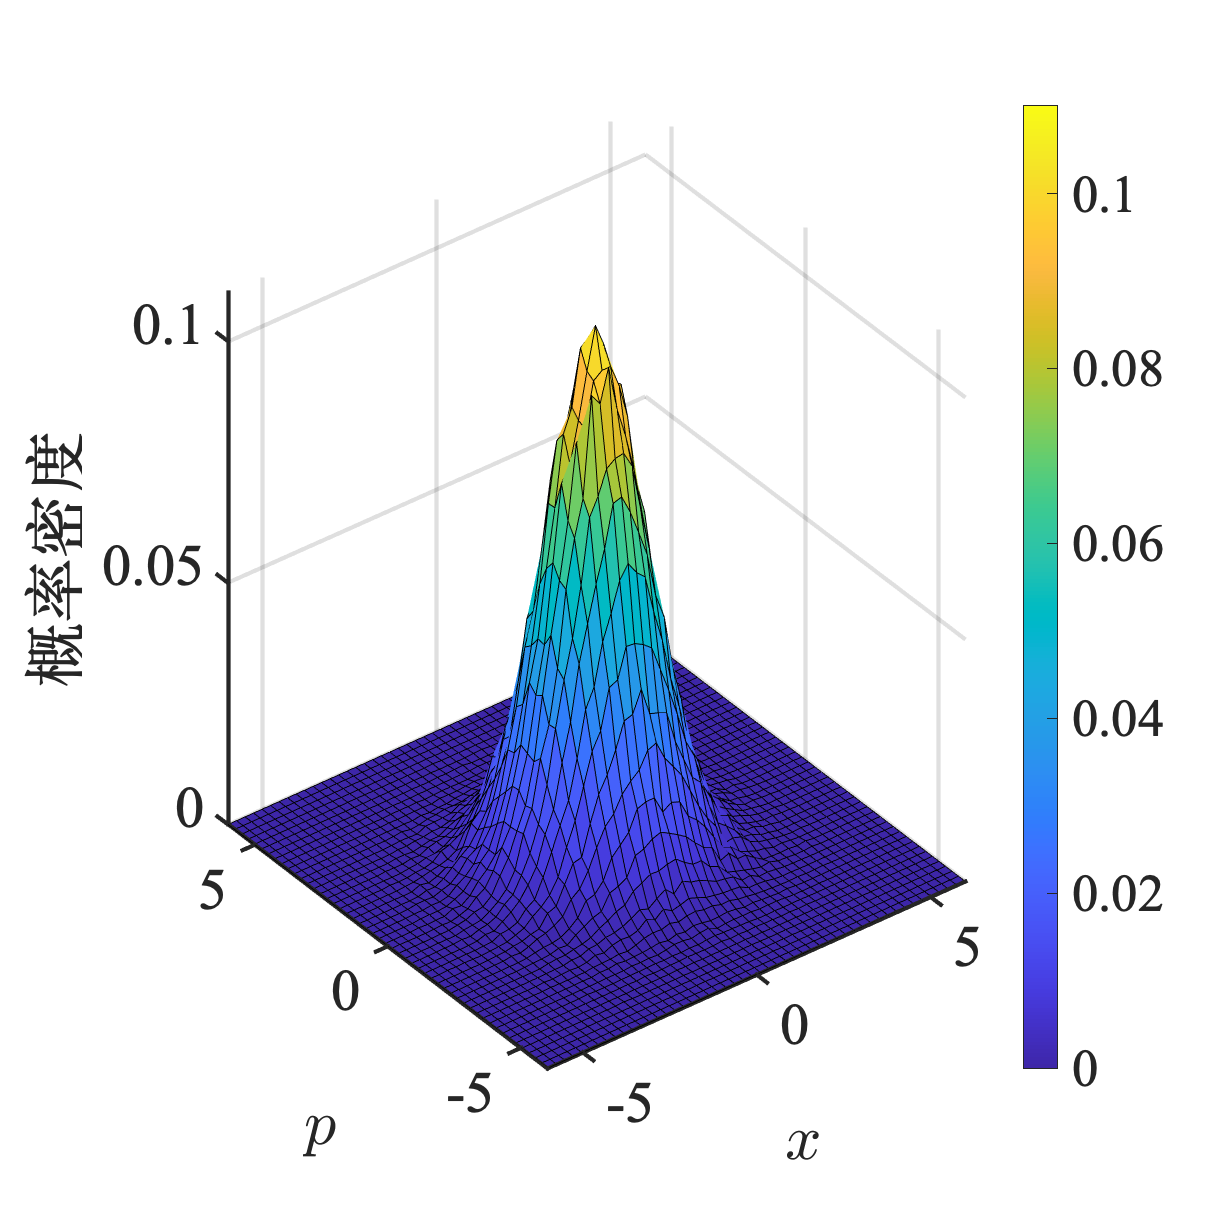
\includegraphics[width=9cm]{2.eps}
	\caption{概率密度图.}
	\label{fig:2}
\end{figure}














% \nocite{*}

\input{bib.tex}

\end{document}
